\chapter{Load Cell Calibration Procedure}

\section{Introduction}

Load cells are essential tools to measuring force in any industrial or
scientific system. One of the most common types of load cells is the strain
gauge load cell. In this type of load cell the deformation of a test material is
measured as a change in the electrical resistance of bonded strain gauge
elements. The test material that the load cell is made of is ideally very rigid,
otherwise significant elastic energy is stored by the load cell and it will
account for a non-negligible amount of deformation in the total system. Large
strains can also permanently damage the load cell by permanently deforming the
load cell or strain gauges and/or breaking the bonding of the load cells to
their substrate.

Here,  I will summarize the load cells used in the biaxial deformation apparatus
and provide a reference for calculations of the predicted load cell response and
calibration procedures. Calibration and verification of that calibration against
the predicted theoretical model is essential to performing accurate experiments
and ensuring that the system is performing as expected and not in need of
further maintenance/repair. 

\section{Calibration procedure}
Calibration of load cells is accomplished with a NIST traceable transfer
calibration standard. The transfer standard is periodically sent out for
recalibration or re-calibrated if it encounters a physical shock such as dropping
or hitting. The transfer standard and load cell are loaded in a series
configuration and the readings of both recorded. From this a calibration curve
can be constructed. The calibration procedure is as follows:

\begin{enumerate}
\item Connect the load cell to the appropriate electronics on the biax (i.e.
    vertical or horizontal axis). Allow a minimum of 30 minutes warm-up to
    ensure that the cell will not drift due to resistive heating from the
    strain gauges. The mechanical installation of the cell and preparation 
    for calibration can take place during warm-up. 
    
\item Plug the 4.5 digit multimeter into the appropriate load cell plugs on the
    biax front panel. 
    
\item  Adjust the zero point of the load cell on the biax control panel. A no-load
    voltage of around -4.5 VDC is best.
    
\item Attach the appropriate ram nose adapter on the vertical hydraulic ram and 
    insert the load cell, gently tightening the set screws. Be sure the cell
    is inserted all the way into the adapter. Attach a DCDT to the adapter and
    connect it.
    
\item Place the proving ring beneath the load cell, centered in both axes. Centering
    is crucial to ensure no damage to the load cell or the proving ring. Be 
    careful, the proving ring is heavy.
    
\item Place a steel loading puck between the proving ring and the load cell. Verify
    that the setup is aligned and that all parts are in-place (Fig.\ref{ring_setup}).

% Figure %
\begin{figure}
	\centering
		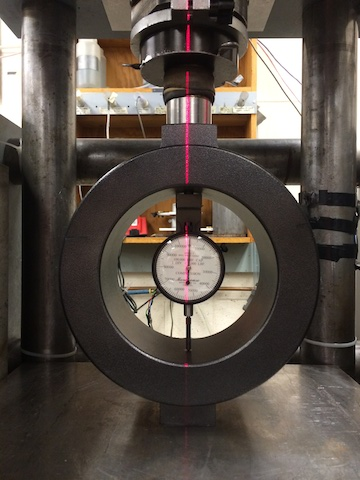
\includegraphics[scale=0.35]{appendix_load_calibration/load_cal.jpg}
   	\caption{A proper setup of the load cell, steel puck, proving ring stack. Notice the careful alignment of all members.}
  	\label{ring_setup}
\end{figure}
% End Figure %

    
\item With the vertical servo control system set to displacement feedback, zero and
    unlock the machine. Be sure you are at the beginning of the displacement 
    range for the DCDT.  

\item Bring the piston down until it is almost touching the proving ring. Check and
    make sure that a DCDT offset isn't needed. Running out of DCDT range during
    calibration will result in severe damage to the proving ring.
    
\item Check the proving ring dial gauge readout. If needed, adjust it to read zero
    klbf (Fig.\ref{ring_zero}).

% Figure %
\begin{figure}
	\centering
		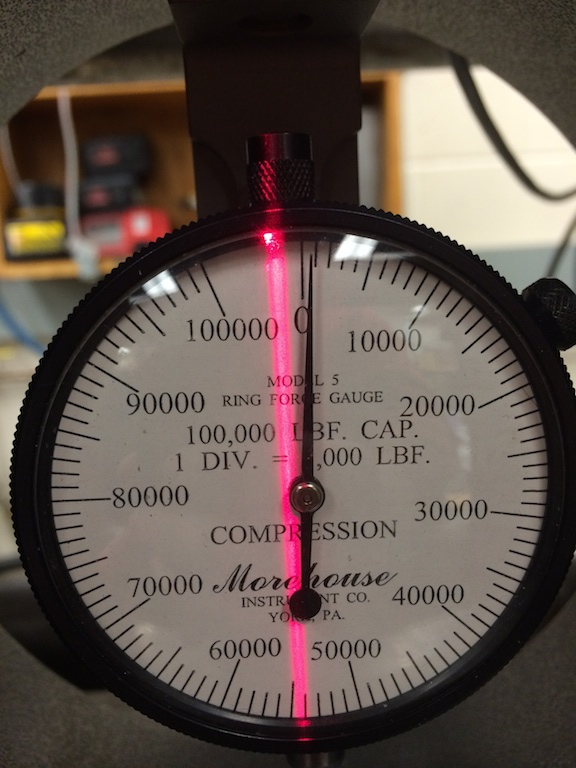
\includegraphics[scale=0.25]{appendix_load_calibration/proving_ring_nozero.jpg}
   	\caption{An example of a proving ring dial under no load that needs adjustment. Simply loosen the dial face set-screw to move the gauge legend.}
  	\label{ring_zero}
\end{figure}
% End Figure %
    
\item Begin recording on the LabView recorder. This data isn't used unless something
    goes wrong, in that case it provides a "black box" style recording of what
    occurred. 
    
\item Set the controller to run the piston downward at 5 um/s. This setting will
     depend on which DCDT you have installed.
     
\item Take a reading at zero load from the panel meter. Record this value.

\item Apply a load to the cell and record the voltage reading. Generally we calibrate low gain biax load cells from 0-65 klbf and high gain from 0-15 klbf. Low stresses should be sampled more often. A common sequence is 0,2.5,5,7.5,10,15,20,25,30,35,...,65 klbf).

\item Repeat step 12 for all loads listed in the loading table. Be sure to not 
     go out of range on the DCDT or load cell.
     
\item Repeat the measurements for all loads during the unloading process as well.
     This characterizes any drift or repeatability issues.
     
\item Convert the loads from klbf to kN. 1 kN = 4.44822162 klbf 

\item Plot the voltage (in mV) and load (in kN). Fit a line. There should not
     be any appreciable non-linear or hysteresis behavior. If there is, consider
     recalibrating or troubleshooting the load cell.

\item Update load cell calibration numbers in the calibration file, logsheets, and your notes.
\end{enumerate}


\section{Typical measured response}

As an example of a typical load cell response, a calibration of the 44mm solid load cell shows a very linear trend with no hysteresis (Fig.\ref{ex_load_cell_fit}).

% Figure %
\begin{figure}
	\centering
		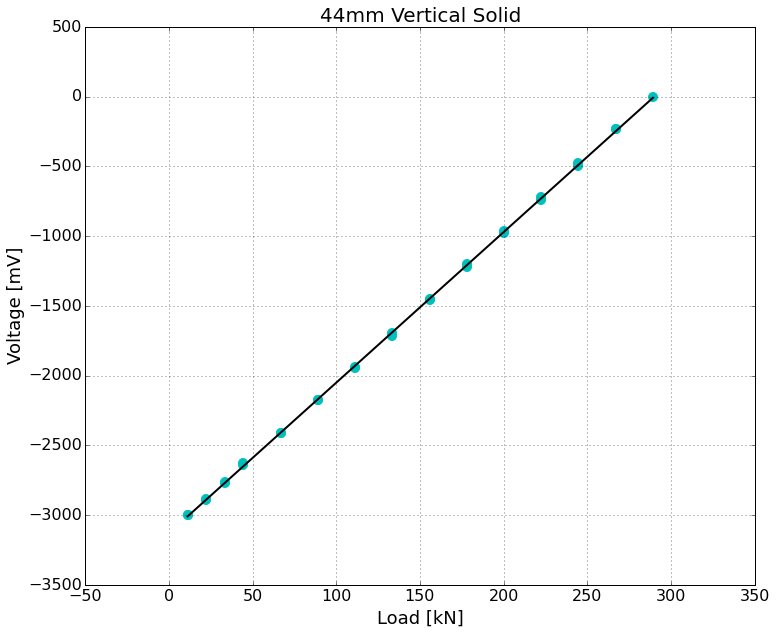
\includegraphics[scale=0.35]{appendix_load_calibration/ex_load_cell_fit.png}
   	\caption{An example calibration obtained from the 44mm solid load cell. }
  	\label{ex_load_cell_fit}
\end{figure}
% End Figure %
